\documentclass[a4paper,10pt]{scrartcl}
\usepackage[margin=2cm,bindingoffset=0cm]{geometry}
\usepackage{ucs}
\usepackage[utf8x]{inputenc}
\usepackage[ngerman]{babel}
\usepackage{fontenc}
%\usepackage[pdftex]{graphicx}
\usepackage{listings}
\usepackage{amssymb}
\usepackage{amsmath}
\usepackage{wasysym}
\usepackage{graphicx}
\usepackage[pdftex]{hyperref}
\author{Verena Käfer (2551188), Niklas Schnelle (2573250), Peter Vollmer (2553704)}
\date{erstellt am 25.10.2010\\
Version: 1.0}
\title{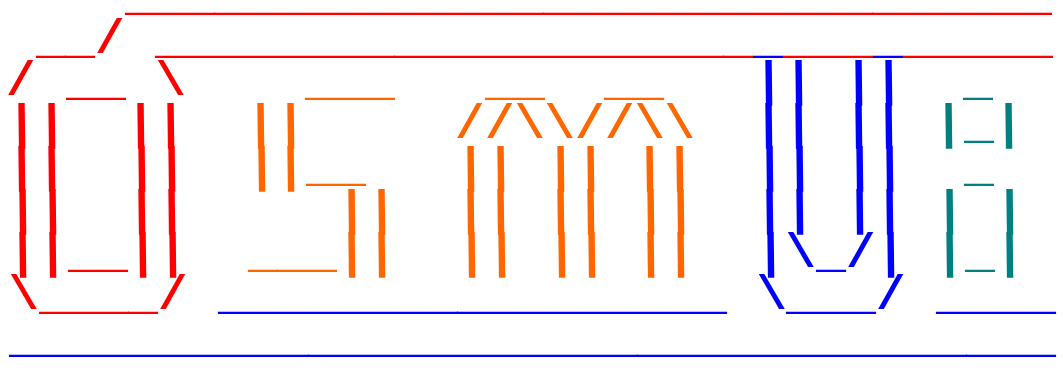
\includegraphics[width=15cm]{../projektplan/Logo_Osmui.png} \\ 
Spezifikation von OsmUi}

\begin{document}
\maketitle
\newpage
\tableofcontents
\newpage

\section{Einleitung}
\subsection{Zweck der Spezifikation}
Bei der Spezifikation handelt es sich um das zentrale Projektdokument. Sie ist Basis aller weiteren Dokumente und
Bezugspunkt in Funktionalitätsfragen. Sie ist daher unbedingt aktuell und konsistent zu halten.\\
Die Spezifikation beschreibt die Funktionen und Anforderungen an das Produkt OsmUi und das zugehörige Projekt.
\subsection{Leserkreis}
Diese Spezifikation richtet sich an:
\begin{itemize}
 \item Die Entwickler von OsmUi
 \item Den Kunden und die Betreuer des SoPra
\end{itemize}

\subsection{Projektüberblick}
In dem Entwicklungsprojekt OsmUi soll eine grafische Benutzeroberfläche für das Kommandozeilenwerkzeug \href{http://wiki.openstreetmap.org/wiki/Osmosis}{Osmosis}
entwickelt werden. Zu diesem Zweck überträgt OsmUi das abstrakte Pipelinekonzept von Osmosis auf eine grafische Darstellung, welche die gesamte Funktionalität von Osmosis zugänglich macht, dabei aber deutlich benutzerfreundlicher sein soll.\\
Während bei Osmosis ein langer Kommandozeilenaufruf eine Pipeline zur Verarbeitung von OpenStreetMap Daten beschreibt, wobei sich der Benutzer die Befehle merken
und korrekt in der gewünschten Reihenfolge aufschreiben muss, soll es mit OsmUi möglich sein eine Verarbeitungspipeline ``zusammen zu klicken''.\\
Hierbei kann die Funktionsweise der einzelnen Tasks sowie deren Interaktion der Benutzeroberfläche von OsmUi entnommen werden.
%\subsection{Konventionen} %Kommt noch

\section{Akteure}
\subsection{Benutzer}
Bei OsmUi gibt es grundsätzlich nur eine Nutzerklasse. Es wird davon ausgegangen, dass OsmUi benutzt wird um eine Verarbeitungspipeline für OpenStreetMap Daten
zu erstellen, welche anschließend durch Osmosis ``ausgeführt'' wird. Hierbei wird davon ausgegangen, dass der Nutzer grundlegende Kentnisse 
von Datenverarbeitung und OpenStreetMap hat.

\section{Nichtfunktionale Anforderungen}
\subsection{Entwurfseinschränkungen}
\subsubsection{Entwurfskonzept}
OsmUi wird nach dem \href{http://de.wikipedia.org/wiki/KISS-Prinzip}{KISS-Prinzip} entwickelt, d.h. entscheidend für die Qualität der Software soll
sein, wie gut die Hauptfunktionen unterstützt werden. Bessere Hauptfunktionalität ist einem größeren Funktionsumfang unterzuordnen.\\
Im Fall von OsmUi heißt dies, dass das Hauptaugenmerk auf dem einfachen und sinnvollen Erstellen von Verarbeitungspipelines, sowie deren Import und Export liegt.\\
Weniger wichtig sind hingegen ``Luxusfunktionen'' wie direktes Anzeigen des Verarbeitungsergebnisses (was auf Grund der Vielfalt der Funktionen von Osmosis
und der Verarbeitungsdauer ohnehin nicht immer sinnvoll ist) oder das direkte Aufrufen von Osmosis.
\subsubsection{Systemumgebung}
Systemumgebung ist das \textbf{Java Runtime Environment in Version 1.6 und höher (SE)}. Dabei ist OsmUi als reine Java Anwendung zu entwickeln, so dass
keine externen Abhängigkeiten bestehen und OsmUi auf allen Java SE kompatiblen Systemen eingesetzt werden kann.
Eventuell wird intern die Bibliothek \textbf{JGraph} eingesetzt, diese wird dann aber direkt mit ausgeliefert
und ist ebenso in platformunabhängigem Java geschrieben. 
\subsubsection{Layout und Gestaltung}
OsmUi soll ab einer Auflösung von 1024x768 benutzbar sein. Alle Fenster sollen, wenn dies sinnvoll ist, skalierbar sein und den eventuell gewonnenen Platz
nutzen. Um Benutzer von Multimonitorsystemen und exotischen Windowmanagern zu entlasten soll die Positionierung von neuen Fenstern nativ erfolgen. Es
sollen insbesondere keine Fenster in eine errechnete Bildschirmmitte von OsmUi positioniert werden.
\subsection{Robustheit}
OsmUi soll als Software möglichst robust arbeiten, d.h. unter allen Bedingungen korrekt arbeiten. Dies soll durch defensive Programmierung erreicht werden.
Jedoch sollen Benutzereingaben möglichst früh geprüft werden, so dass tiefere Funktionen den Daten ``vertrauen'' können. Dies sichert zudem ab, dass klar ist, welcher
Programmteil für die Prüfung zuständig ist. Nämlich immer der erste, der die nötigen Informationen hat.\\
Weiterhin wird die Robustheit durch das KISS-Prinzip unterstützt, da weniger Funktionen besser entworfen und getestet werden können.
\subsection{Portabilität}
OsmUi soll durch den Einsatz reinen Javas auf allen Systemen mit Java SE 1.6 Unterstützung lauffähig sein. Als Exportformate für Osmosis Aufrufskripte
werden .bat und .sh (/bin/sh) unterstützt, womit alle Posix Systeme sowie Windows abgedeckt sind.
\subsection{Erweiterbarkeit}
Das Programm muss keine besonderen Erweiterungsfunktionalitäten wie etwa ein Pluginsystem zur Verfügung stellen, jedoch werden der Programmcode und die Systemarchitektur
so gestaltet, dass OsmUi leicht und schnell an neue oder veränderte Osmosis Funktionen angepasst werden kann.
\section{Distributionsform und Installation}
OsmUi wird als ausführbares JAR Archiv ausgeliefert, welches direkt ausgeführt werden kann.


\section{Funktionale Anforderungen}
\subsection{Mengengerüst}
Bei OsmUi handelt es sich um eine Einzelplatzanwendung und es wird keine Netzwerkfunktion genutzt, somit gibt es zu jedem Zeitpunkt genau einen Nutzer.\\
Beim Erstellen/Laden/Speichern von Verarbeitungspipelines muss OsmUi in der Lage sein, mit Pipelines von bis zu 100 Tasks zuverlässig zu arbeiten -
eine künstliche Beschränkung nach oben besteht jedoch nicht.
\subsection{Laden und Speichern von Verarbeitungspiplines als Osmosis Aufrufscript}
Dem KISS-Prinzip folgend bietet OsmUi eine einheitliche Laden- und Speichern-Funktion, die sowohl bereits vorhandene Osmosis Aufrufscripts als auch durch OsmUi
selbst erstellte Verarbeitungspiplines, laden kann. Die Speicherung erfolgt als Osmosis Aufrufskripte.\\
Dies ermöglicht auch beim Wechsel des Werkzeugs einen leichten Zugriff auf alle mit OsmUi erstellten Dateien.
\subsubsection{Laden}
Eine der Hauptfunktionen von OsmUi stellt das Laden von Aufrufscripten dar. Dabei können sowohl Dateien im .bat - als auch im .sh Format (mit \#!/bin/sh Shebang),
sowie Textdateien, in denen nur eine Osmosis Parameterliste steht, geladen werden. Sie werden direkt im Pipelinebearbeitungsfeld angezeigt und
stehen zur Bearbeitung bereit.
\subsubsection{Speichern}
Zum Speichern wählt der Benutzer entweder einen neue Datei aus, die, wenn vorhanden, überschrieben und sonst neu erstellt wird. Oder er überschreibt die gerade bearbeitete Datei.
Der Dateityp kann hierbei zwischen .sh Script und .bat gewählt werden.
\subsection{Benutzeroberfläche}
Die Benutzeroberfläche von OsmUi ist in zwei Teile aufgeteilt: die Taskauswahlbox und die Pipelinebox. Desweiteren gibt es ein Anwendungsmenü und beim Bearbeiten eines Tasks
wird es ein weiteres Einstellungsfenster geben.
\subsubsection{Taskauswahlbox}
Im linken Teil der Benutzeroberfläche wird eine Liste der gerade zum Einfügen verfügbaren Tasks dargestellt. Dabei kann die Darstellung als Icon,
Text oder Kombination erfolgen. Es werden nur Tasks angezeigt die gerade auch einfügbar sind. \\
Am Anfang sind dies zum Beispiel alle Tasks, (z.B. read XML) die keinen Streameingang haben. Ist in der Pipelinebox ein Task ausgewählt, so
sind nur diejenigen Tasks sichtbar, die mit dem/den Ausgang/Ausgängen des ausgewählten Task kompatibel sind.\\
So wird verhindert, dass der Benutzer Pipelines bauen kann, die nicht durch Osmosis ausführbar sind.
\subsubsection{Pipelinebox}
In der Pipelinebox wird die Pipeline grafisch dargestellt und es können Tasks zum Bearbeiten ausgewählt werden. Ist ein Task ausgewählt so können seine Eigenschaften
bearbeitet oder ein neuer Task über die Taskauswahlbox - wie oben beschrieben - angefügt werden. Desweiteren kann eine Verbindung zu einem anderen Task, der noch offene
Inputs hat, hergestellt werden.
\subsubsection{Taskeinstellungsdialog}
Wählt der Benutzer einen Task aus, so stellt OsmUi einen Dialog zur Verfügung, in dem alle - für den jeweiligen Tasktyp vorhandenen - Parameter eingegeben werden können.
Hierbei kann die Eingabe eingeschränkt sein: als Spanne von Zahlen, als Kartenausschnitt oder als freier Text erfolgen. Dabei wird der für
den Datentyp beste Eingabemodus gewählt.
\subsubsection{Lokalisation}
OsmUi wird eine übersetzte Benutzeroberfláche für mindestens die Sprachen Deutsch und Englisch bieten. Dabei wird die aktuell verwendete
Sprache aus den hierfür vorgesehenen Umgebungsvariablen eingelesen, um sie ohne Interaktion durch den Benutzer in dessen System einzugliedern.

\subsection{Use Cases}

\begin{tabular}{|p{5cm}|p{10cm}|}
\hline Name & Datei laden \\ 
\hline Ziel & gespeicherte Datei soll geladen werden \\ 
\hline Vorbedingung & Eine gespeicherte Datei ist vorhanden \\ 
\hline Nachbedingung & Die Datei wurde geladen \\ 
\hline Nachbedingung im Sonderfall & Es wurde nichts geladen \\ 
\hline Akteure & Benutzer \\ 
\hline Normalablauf & - Der Benutzer klickt auf den Lade-Button
\newline 
- Das Lade-Menü öffnet sich
\newline 
- Der Benutzer wählt die gewünschte Datei aus
\newline 
- Die gewählte Datei wird geladen
\\ 
\hline Sonderfall &  
 - Der Benutzer klickt auf den Lade-Button
 \newline
 - Das Lade-Menü öffnet sich
 \newline
 - Der Benutzer hat noch nichts gespeichert oder will nichts laden
 \newline
 - Der Benutzter bricht den Vorgang ab
\\
\hline 
\end{tabular} 
\\
\\
\begin{tabular}{|p{5cm}|p{10cm}|}
\hline Name & Datei speichern \\ 
\hline Ziel & Aktuelle Datei soll gespeichert werden \\ 
\hline Vorbedingung & Die aktuelle Datei wurde schon einmal gespeichert \\ 
\hline Nachbedingung & Die Datei wurde gespeichert \\ 
\hline Nachbedingung im Sonderfall 1) & Die Datei wurde neu gespeichert \\ 
\hline Nachbedingung im Sonderfall 2) & Die Datei wurde nicht gespeichert\\
\hline Akteur & Benutzer \\ 
\hline Normalablauf & - Der Benutzer klickt den Speicher-Button 
\newline
- Die Datei wird gespeichert
\\
\hline Sonderfall 1) & - Der Benutzer klickt auf den Speicher-Button
\newline
- Das Speichern-unter-Menü öffnet sich
\newline
- weiter wie im Use-Case Datei speichern unter
 \\ 
 \hline Sonderfall 2) & - Der Benutzer bricht den vorgang ab \\
\hline 
\end{tabular} 
\\
\\
\begin{tabular}{|p{5cm}|p{10cm}|}
\hline Name & Datei speichern unter \\ 
\hline Ziel & Die Datei soll in einem selbst gewählten Verzeichnis gespeichert werden \\ 
\hline Vorbedingung & keine \\ 
\hline Nachbedingung & Die Datei wurde im gewählten Verzeichnis gespeichert \\ 
\hline Nachbedingung im Sonderfall & Die Datei wurde nicht gespeichert \\ 
\hline Akteur & Benutzer \\ 
\hline Normalablauf & - Der Benutzer klickt den Speichern-unter-Button
\newline 
- Das Speichern-unter-Menü öffnet sich
\newline
- Der Benutzer wählt den Speicherort und den Namen
\newline
- Die Datei wird gespeichert
\\ 
\hline Sonderfall & - Der Benutzer bricht den Vorgang ab \\ 
\hline 
\end{tabular} 
\\
\\
\begin{tabular}{|p{5cm}|p{10cm}|}
\hline Name & Hilfe aufrufen \\ 
\hline Ziel & Das Hilfe-Menü soll aufgerufen werden \\ 
\hline Vorbedingung & keine \\ 
\hline Nachbedingung & Das Hilfe-Menü wurde geöffnet \\ 
\hline Akteur & Benutzer \\ 
\hline Normalablauf & - Der Benutzer klickt den Hilfe-Button
\newline
- Das Hilfe-Menü wurde geöffnet \\ 
\hline 
\end{tabular} 
\\
\\
\begin{tabular}{|p{5cm}|p{10cm}|}
\hline Name & neue Datei erstellen \\ 
\hline Ziel & Eine neue Datei soll erstellt werden \\ 
\hline Vorbedingung & keine \\ 
\hline Nachbedingung & Eine neue Datei wurde erstellt \\ 
\hline Akteur & Benutzer \\ 
\hline Normalablauf & - Der Benutzer klickt den Neu-Datei-erstellen-Button
\newline
- Eine neue Datei öffnet sich
\\ 
\hline 
\end{tabular} 
\\
\\
\begin{tabular}{|p{5cm}|p{10cm}|}
\hline Name & neuen Task hinzufügen \\ 
\hline Ziel & Ein neuer Task soll hinzugefügt werden \\ 
\hline Vorbedingung & keine \\ 
\hline Nachbedingung & Ein neuer Task wurde hinzugefügt \\ 
\hline Akteur & Benutzer \\ 
\hline Normalablauf & - Der Benutzer wählt einen neuen Task aus und setzt die Einstellungen
\newline
- Der Task wird hinzugefügt
\\ 
\hline 
\end{tabular}
\\
\\
\begin{tabular}{|p{5cm}|p{10cm}|}
\hline Name & Task entfernen \\ 
\hline Ziel & Ein Task soll entfernt werden \\ 
\hline Vorbedingung & Es ist mindestens ein Task vorhanden \\ 
\hline Nachbedingung & Der Task wurde gelöscht \\ 
\hline Nachbedingung im Sonderfall & Eine Warnung wurde ausgsgeben \\ 
\hline Akteur & Benutzer \\ 
\hline Normalablauf & - Der Benutzer wählt den zu löschenden Task aus und klickt den Löschen-Button
\newline
- Der Task wird gelöscht
\\ 
\hline Sonderfall & - Der Benutzer wählt den zu löschenden Task und klickt den Löschen-Button
\newline
- OsmUi gibt eine Warnung aus und der Task wird gelöscht
 \\ 
\hline 
\end{tabular}  
\\
\\\begin{tabular}{|p{5cm}|p{10cm}|}
\hline Name & Task ändern \\ 
\hline Ziel & Ein bestehender Task soll geändert werden \\ 
\hline Vorbedingung & Es gibt mindestens einen Task \\ 
\hline Nachbedingung & Der Task wurde geändert \\  
\hline Akteur & Benutzer \\ 
\hline Normalablauf & - Der Benutzer wählt den zu ändernden Task an und klickt den Ändern-Button
\newline
- Der Benutzer ändert die gewünschten Eigenschaften und klickt auf den OK-Button
\\ 
\hline 
\end{tabular} 


\subsection{Begriffslexikon}

\begin{tabular}{|p{5cm}|p{10cm}|}
\hline Begriff & Task \\ 
\hline Bedeutung & Ist ein Bearbeitungsschritt einer Pipeline\\ 
\hline Abgrenzung & Ein Task ist kein Parameter, er besitzt diese. Ein Task ist keine Anwendung/Aufgabe im herkömmlichen Sinne \\ 
\hline Gültigkeit & Ist nur gültig für das Pipelinesystem von Osmosis. \\ 
\hline Bezeichnung & Ein Task ist für eine eindeutigen Bearbeitungsschritt von Osmosis zuständig\\ 
\hline Unklarheiten & Keine \\ 
\hline Querverweise & Parameter\\ 
\hline 
\end{tabular}
\\
\begin{tabular}{|p{5cm}|p{10cm}|}
\hline Begriff & Pipeline \\ 
\hline Bedeutung & Eine Pipeline ist ein Konstrukt, dem Daten zugeführt werden, diese bearbeitet und anschließend zurückgibt.  \\ 
\hline Abgrenzung & Eine Pipeline kein reales Rohrsysteme gemeint. Es sind reine Gedanken-Konstrukte \\ 
\hline Gültigkeit & Die Bedeutung des Wortes verfäll ausßerhalb von Osmosis. \\ 
\hline Bezeichnung & Eine Pipeline ist durch die in ihr enthaltenen Tasks eindeutig bestimmt \\ 
\hline Unklarheiten & keine \\ 
\hline Querverweise & Task \\ 
\hline 
\end{tabular}
\\
\begin{tabular}{|p{5cm}|p{10cm}|}
\hline Begriff & Aufrufscript \\ 
\hline Bedeutung &  \\ 
\hline Abgrenzung &  \\ 
\hline Gültigkeit &  \\ 
\hline Bezeichnung &  \\ 
\hline Unklarheiten &  \\ 
\hline Querverweise &  \\ 
\hline 
\end{tabular}
\\
\begin{tabular}{|p{5cm}|p{10cm}|}
\hline Begriff & Pipelinebox \\ 
\hline Bedeutung & Ist der Teil der Oberfläche, in der die Pipeline grafisch dargestellt wird. \\ 
\hline Abgrenzung & Es handelt sich um keine reale Box, sondern um ein gedankliches Konstrukt \\ 
\hline Gültigkeit & Der Begriff gilt innerhalb von Osmosis \\ 
\hline Bezeichnung & es gibt nur eine Pipelinebox \\ 
\hline Unklarheiten & keine \\ 
\hline Querverweise & Pipeline \\ 
\hline 
\end{tabular}
\\
\begin{tabular}{|p{5cm}|p{10cm}|}
\hline Begriff &  \\ 
\hline Bedeutung &  \\ 
\hline Abgrenzung &  \\ 
\hline Gültigkeit &  \\ 
\hline Bezeichnung &  \\ 
\hline Unklarheiten &  \\ 
\hline Querverweise &  \\ 
\hline 
\end{tabular}
\\
\begin{tabular}{|p{5cm}|p{10cm}|}
\hline Begriff &  \\ 
\hline Bedeutung &  \\ 
\hline Abgrenzung &  \\ 
\hline Gültigkeit &  \\ 
\hline Bezeichnung &  \\ 
\hline Unklarheiten &  \\ 
\hline Querverweise &  \\ 
\hline 
\end{tabular}
\end{document}
